El presente capítulo documenta los resultados correspondientes al desarrollo e implementación del prototipo FLP Viewer, en cumplimiento del objetivo específico 4 del proyecto. El capítulo se organiza en seis secciones. En primer lugar, se describe el repositorio de código fuente y su estructura de directorios. En segundo lugar, se detallan los componentes implementados, abordando el pipeline de gramática, la arquitectura del cliente, la biblioteca de ejemplos predefinidos, el punto de acceso de ejecución y la instrumentación en tiempo de ejecución. En tercer lugar, se presenta el flujo principal de ejecución a través de un diagrama de secuencia. En cuarto lugar, se describe la configuración de despliegue en el entorno de pruebas. En quinto lugar, se verifica el cumplimiento de los requisitos funcionales definidos en el diseño. Finalmente, se presenta la evaluación de la calidad del software mediante análisis estático del código fuente.

\section{Repositorio de código fuente}

El código fuente del prototipo se encuentra alojado en el repositorio público de GitHub disponible en \url{https://github.com/Esmeralda-RG/flp-viewer}. El repositorio registra el historial completo de \textit{commits} del proceso de desarrollo, organizado en torno a las funcionalidades incrementales del sistema. El archivo \texttt{README.md} incluye la descripción del proyecto, el stack tecnológico utilizado, las instrucciones de instalación y ejecución local, la estrategia de integración con Racket y la descripción de la estructura de directorios.

La estructura del proyecto sigue la convención del \textit{App Router}\footnote{El \textit{App Router} es el sistema de enrutamiento de Next.js basado en el sistema de archivos introducido en la versión 13. Organiza las rutas, los componentes de servidor y la lógica de la API dentro del directorio \texttt{app/}, permitiendo mezclar componentes de servidor y de cliente en la misma aplicación.} de Next.js \cite{nextjs}, con los siguientes directorios principales:

\begin{itemize}
  \item \texttt{app/api/run/}: contiene la ruta de API encargada de gestionar la ejecución del intérprete Racket, junto con los archivos \texttt{.rkt} de instrumentación en tiempo de ejecución (\texttt{\_runner.rkt}, \texttt{\_tracking.rkt} y \texttt{\_stream-parser.rkt}).
  \item \texttt{app/components/}: agrupa los componentes de la interfaz de usuario, entre ellos el orquestador \texttt{PlaygroundLayout}, el visualizador de árbol \texttt{ASTViewer}, el panel de ambiente \texttt{EnvironmentPanel}, la consola \texttt{ConsoleOutput}, el editor \texttt{EditorPanel} y los modales auxiliares.
  \item \texttt{app/lib/}: contiene los módulos del pipeline de gramática, los generadores de código Racket y las utilidades del playground.
  \item \texttt{app/services/}: incluye el cliente HTTP que comunica la capa cliente con la ruta de API.
  \item \texttt{app/types/}: centraliza las definiciones de tipos TypeScript compartidas entre módulos.
  \item \texttt{examples/}: almacena las plantillas de programas predefinidos cargadas en el renderizado inicial del servidor.
\end{itemize}


\section{Implementación de los componentes}

\subsection{Pipeline de gramática BNF}

El pipeline de gramática se implementó íntegramente en TypeScript \cite{typescript} como una cadena de módulos independientes que opera en el cliente sin intervención del servidor. Su punto de entrada único es la función \texttt{runPipeline}, definida en \texttt{grammar-pipeline.ts}, que recibe la especificación léxica y la gramática en notación BNF y retorna los archivos del intérprete generados o una lista de errores.

La cadena de transformación sigue el modelo clásico de compilación \cite{aho2006compilers} y comprende tres etapas secuenciales, ilustradas en la figura~\ref{fig:pipeline-gramatica}. La primera es el análisis léxico, implementado en \texttt{bnf-lexer.ts}: la función \texttt{tokenize} recorre el texto de entrada carácter a carácter y produce una secuencia de tokens tipados. La segunda es el análisis sintáctico, implementado en \texttt{bnf-parser.ts}: la función \texttt{parse} consume la secuencia de tokens y construye una representación intermedia de la gramática (\texttt{GrammarAST}) compuesta por reglas de producción. Los errores de ambas etapas se reportan mediante las clases \texttt{LexError} y \texttt{ParseError}, respectivamente, ambas con la línea y columna exactas del fallo. La tercera etapa es la generación de código, distribuida en tres módulos especializados que consumen el \texttt{GrammarAST} de forma independiente. \texttt{eopl-generator.ts} produce el archivo \texttt{grammar.rkt} con la especificación léxica y gramatical en formato SLLGEN. \texttt{env-generator.ts} genera \texttt{environment.rkt} con el ambiente inicial y las funciones de extensión. \texttt{main-generator.ts} produce \texttt{main.rkt} con los \textit{stubs}\footnote{Un \textit{stub} es una función con cuerpo incompleto que declara la firma esperada y sirve como marcador del trabajo pendiente de implementación. En este contexto, los \textit{stubs} definen las funciones de evaluación del intérprete que el estudiante debe completar.} de las funciones de evaluación pendientes de implementación por parte del estudiante, registrando además las líneas bloqueadas para protección en el editor.

\begin{figure}[htbp]
\centering
\resizebox{\textwidth}{!}{\begin{tikzpicture}[
    node distance=1.1cm and 0.9cm,
    box/.style={
        rectangle, rounded corners=4pt,
        draw=SteelBlue, fill=SteelBlue!10,
        text width=2.3cm, align=center,
        minimum height=1.1cm,
        font=\small, inner sep=4pt
    },
    file/.style={
        rectangle, rounded corners=4pt,
        draw=gray!60, fill=gray!8,
        minimum width=2.6cm, minimum height=0.9cm,
        align=center, font=\small\ttfamily, inner sep=4pt
    },
    arr/.style={->, >=Stealth, thick, draw=gray!60},
    lbl/.style={font=\scriptsize\itshape, fill=white, inner sep=1pt}
]
    % Fila superior: especificación, análisis léxico y sintáctico
    \node[box] (input) {Especificación\\léxica + BNF};
    \node[box, right=of input] (lex)   {Análisis\\léxico};
    \node[box, right=of lex]   (parse) {Análisis\\sintáctico};

    % Representación intermedia, centrada bajo la fila superior
    \node[box, below=1.5cm of lex] (ast) {Representación\\intermedia};

    % Generación de código, centrada bajo la representación intermedia
    \node[box, below=1.3cm of ast] (codegen) {Generación\\de código};

    % Archivos Racket generados
    \node[file, below=1.3cm of codegen] (envrkt)     {environment.rkt};
    \node[file, left=1.0cm of envrkt]   (grammarrkt) {grammar.rkt};
    \node[file, right=1.0cm of envrkt]  (mainrkt)    {main.rkt};

    % Flechas fila superior
    \draw[arr] (input) -- (lex);
    \draw[arr] (lex)   -- node[above, lbl] {tokens} (parse);

    % La sintaxis analizada produce la representación intermedia
    \draw[arr] (parse.south) -- ++(0,-0.5) -| node[above, near start, lbl] {produce} (ast.north);

    % La representación intermedia alimenta la generación de código
    \draw[arr] (ast) -- (codegen);

    % La generación de código produce los tres archivos Racket
    \draw[arr] (codegen.south) -- (envrkt.north);
    \draw[arr] (codegen.south) -- ++(0,-0.6) -| (grammarrkt.north);
    \draw[arr] (codegen.south) -- ++(0,-0.6) -| (mainrkt.north);
\end{tikzpicture}
}
\caption{Pipeline de gramática BNF: de la especificación de entrada a los archivos Racket generados, pasando por el análisis léxico, el análisis sintáctico y la generación de código.}
\label{fig:pipeline-gramatica}
\end{figure}

La especificación léxica se define en un área de texto independiente del modal de gramática, escribiendo un nombre de token por línea. Para cada nombre reconocido (\texttt{number}, \texttt{float}, \texttt{identifier}, \texttt{binary}, \texttt{octal}, \texttt{hex} y \texttt{text}) la función \texttt{expandLexRule} de \texttt{eopl-generator.ts} produce las reglas SLLGEN correspondientes. Las reglas de espaciado (\texttt{whitespace}) y de comentarios de línea (\texttt{comment}) se incluyen siempre de forma automática. Si el área léxica se deja vacía, el pipeline incorpora el conjunto completo de tokens por defecto. Para tipos léxicos no contemplados en los nombres predefinidos, el estudiante puede escribir directamente la regla en notación SLLGEN entre paréntesis, que el pipeline incorpora sin transformaciones.

\subsection{Componente orquestador y paneles de la interfaz}

La Figura \ref{fig:bienvenida} muestra el modal de bienvenida que se presenta al estudiante en el primer acceso. El modal ofrece un resumen de las acciones básicas y carga automáticamente el ejemplo \textit{Hola Mundo} como punto de partida.

\begin{figure}[H]
    \centering
    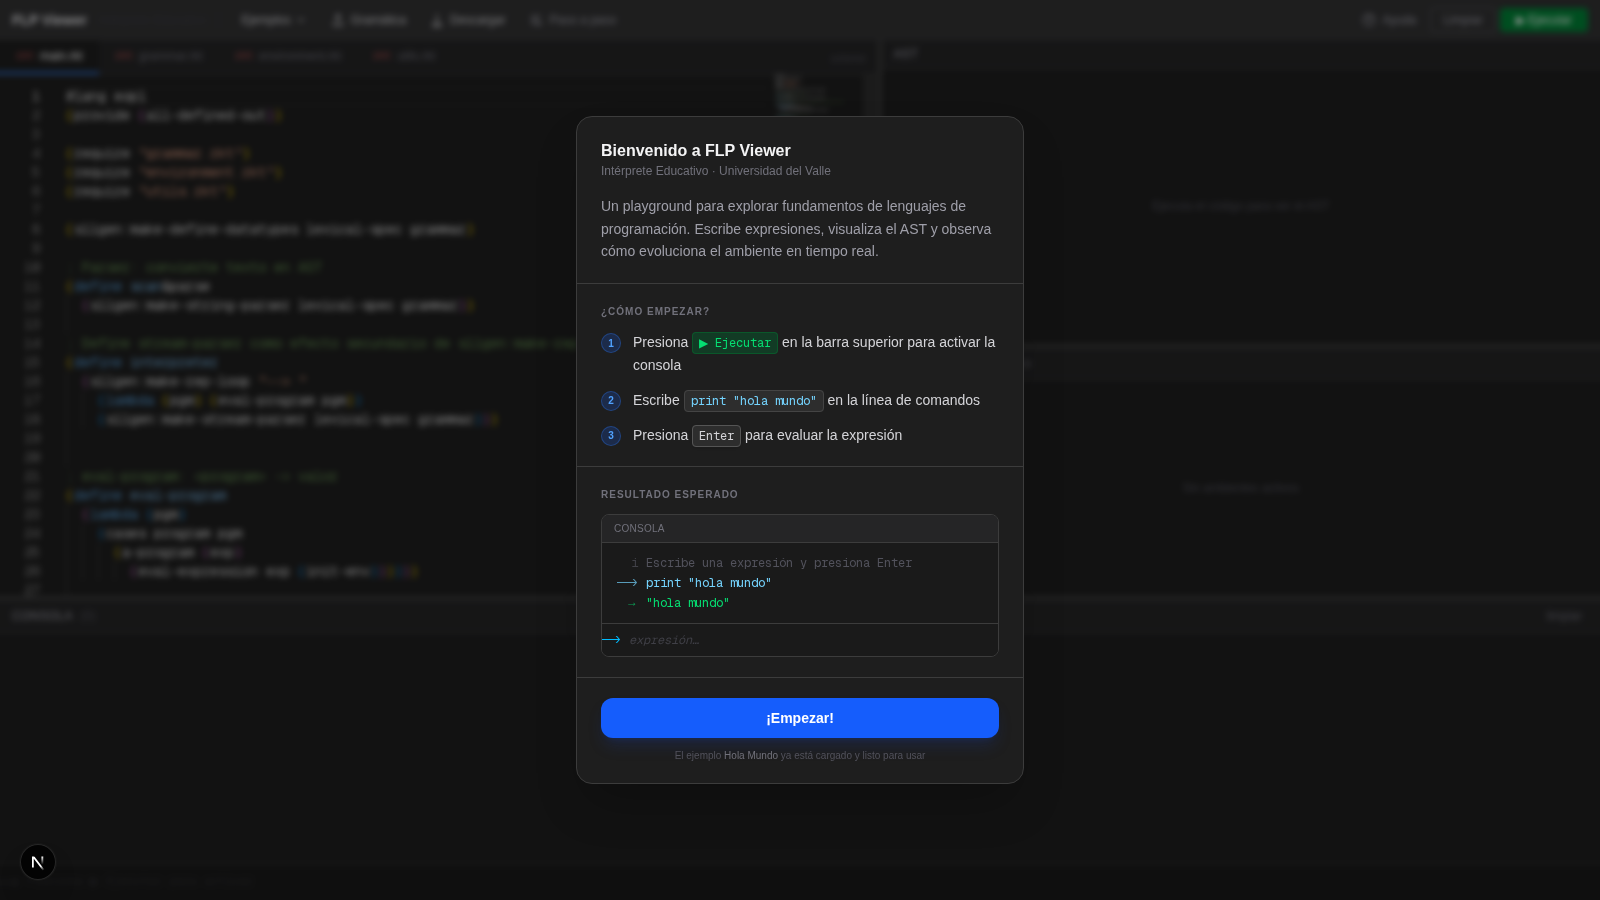
\includegraphics[width=\textwidth]{Capitulo_5/imagenes/cap-01-bienvenida.png}
    \caption{Modal de bienvenida del prototipo FLP Viewer}
    \scriptsize \textbf{Fuente:} Elaboración propia
    \label{fig:bienvenida}
\end{figure}

\FloatBarrier

El componente \texttt{PlaygroundLayout} actúa como orquestador central de la interfaz. Mantiene el estado global de la sesión de trabajo e implementa las transiciones de estado definidas en el diseño: inicio y fin de ejecución, recepción de resultados, avance paso a paso y apertura de modales auxiliares.

El estado que gestiona el orquestador comprende los archivos del editor (\texttt{files}), el árbol de sintaxis abstracta activo (\texttt{ast}), los marcos del ambiente de ejecución (\texttt{frames}), el historial de mensajes de la consola (\texttt{logs}), los indicadores de sesión activa y ejecución en curso, el modo de evaluación paso a paso (\texttt{stepMode}) y la cola de pasos pendientes (\texttt{pendingSteps}). Los cuatro paneles de visualización (\texttt{ASTViewer}, \texttt{EnvironmentPanel}, \texttt{ConsoleOutput} y \texttt{EditorPanel}) son componentes React \cite{react} sin estado propio: reciben exclusivamente los datos necesarios para su renderizado a través de las propiedades que el orquestador les suministra.

El modo de evaluación paso a paso opera mediante una cola de pasos (\texttt{pendingSteps}) que se inicializa con el resultado retornado por la API para cada expresión de nivel superior enviada por el estudiante. Cada vez que el usuario activa el control \textit{Next step}, el orquestador extrae el siguiente paso de la cola y actualiza de forma sincronizada el árbol AST, los marcos del ambiente y la salida de la consola, mostrando el resultado de la expresión correspondiente a ese paso de forma aislada, sin conservar las ligaduras de las expresiones anteriores, con la granularidad descrita en el Capítulo~\ref{cap4}.

La Figura \ref{fig:paso-a-paso} ilustra la interfaz en modo paso a paso, con el botón de avance visible en la consola y el estado del AST y el ambiente correspondiente al paso activo.

\begin{figure}[H]
    \centering
    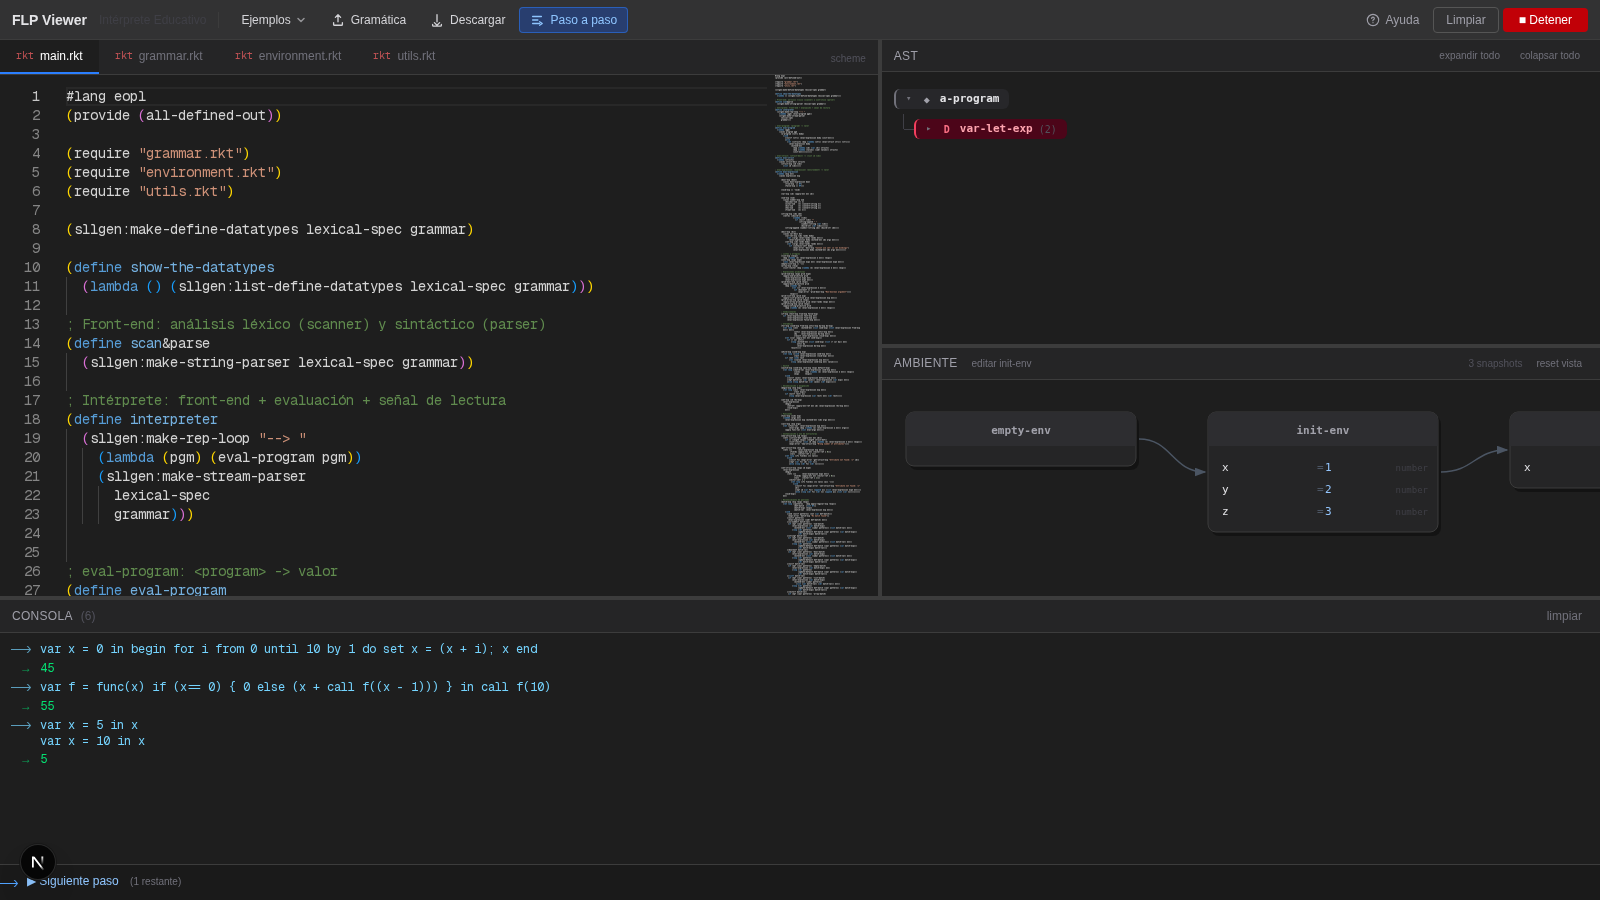
\includegraphics[width=\textwidth]{Capitulo_5/imagenes/cap-08-paso-a-paso.png}
    \caption{Modo de evaluación paso a paso con pasos pendientes de navegación}
    \scriptsize \textbf{Fuente:} Elaboración propia
    \label{fig:paso-a-paso}
\end{figure}

\FloatBarrier

La Figura \ref{fig:modal-gramatica} ilustra el modal de definición de gramática con una especificación BNF y la vista previa del archivo \texttt{grammar.rkt} generado.

\begin{figure}[H]
    \centering
    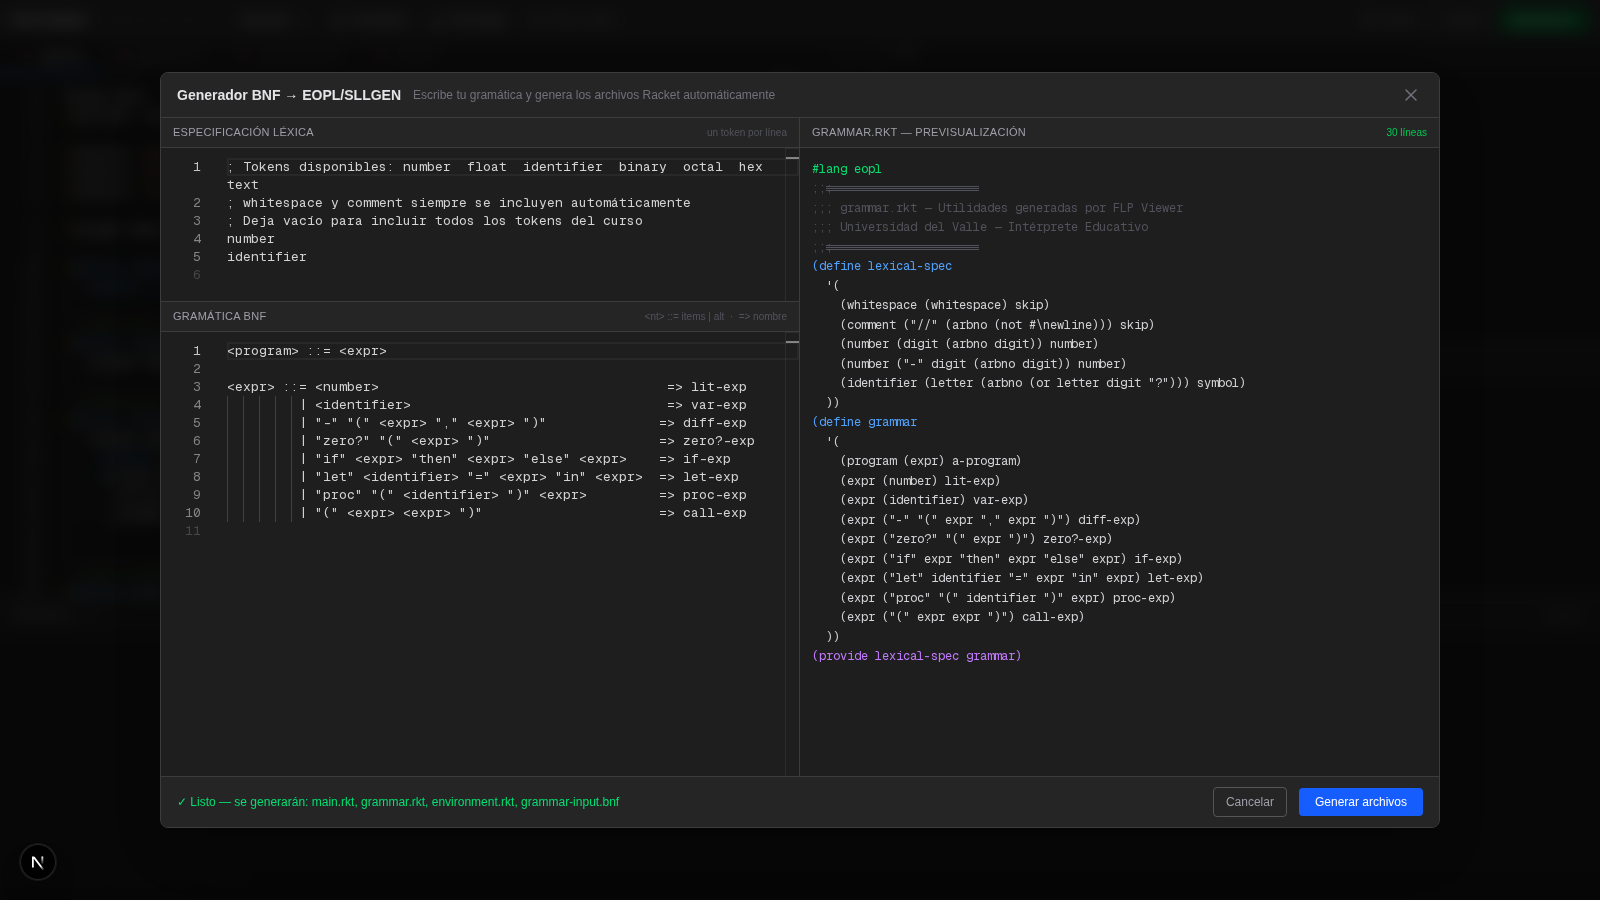
\includegraphics[width=\textwidth]{Capitulo_5/imagenes/cap-05-modal-gramatica.png}
    \caption{Modal de definición de gramática BNF con vista previa del archivo generado}
    \scriptsize \textbf{Fuente:} Elaboración propia
    \label{fig:modal-gramatica}
\end{figure}

\FloatBarrier

El modal de gramática (\texttt{GrammarModal}) recibe las entradas del estudiante y, al confirmar, invoca \texttt{runPipeline} para obtener los archivos generados, que son cargados en el panel de edición a través del mecanismo \texttt{upsertFile}. Si el pipeline reporta errores léxicos o sintácticos, estos se presentan en el modal antes de cerrar, sin modificar los archivos activos en el editor.

El componente \texttt{EditorPanel} utiliza Monaco Editor \cite{monaco} para la edición de código. Las líneas generadas automáticamente por el pipeline se marcan como de solo lectura mediante la API de rangos de Monaco, de modo que el estudiante solo puede editar las secciones correspondientes a la lógica de evaluación.

Las Figuras~\ref{fig:interfaz-principal} y~\ref{fig:eval-cierres} documentan dos evaluaciones representativas sobre el ejemplo \textit{Intérprete EOPL (avanzado)}, seleccionadas por su correspondencia directa con los indicadores de logro IL~1.2.6 e IL~1.2.7, identificados en el Capítulo~\ref{cap3} como las fuentes de mayor dificultad conceptual del R.A.2 (Tabla~\ref{tabla:indicadores_logro_prototipo}). Dicho resultado concentra el 50.0\,\% del peso evaluativo de la asignatura, y el 77.8\,\% de los estudiantes encuestados reportó haber tenido dificultades con los conceptos asociados (entornos, estado y secuenciación) durante su cursada (P4, Tabla~\ref{tabla:encuesta_estudiantes}). Las evaluaciones cubren, de forma complementaria, los dos ejes semánticos que el diagnóstico identificó como prioritarios: el estado mutable con iteración, cuya comprensión exige distinguir entre ligadura y asignación destructiva (IL~1.2.7), y las funciones de orden superior con clausuras, cuya representación hace visible cómo el ambiente registra procedimientos como valores de primera clase almacenados junto a cualquier otra ligadura (IL~1.2.6) \cite{Friedman2008EPL}.

La Figura \ref{fig:interfaz-principal} evalúa la expresión \texttt{var x = 0 in begin for i from 0 until 10 by 1 do set x = (x + i); x end}, que acumula la suma de 0 a 9 mediante un bucle con asignación destructiva. El panel de ambiente muestra la cadena \texttt{empty-env} $\to$ \texttt{init-env} $\to$ \texttt{x}, donde el marco final refleja el valor de \texttt{x} tras la última iteración del bucle. Este caso documenta que la instrumentación captura correctamente la evolución del estado mutable a lo largo de la ejecución.

\begin{figure}[H]
    \centering
    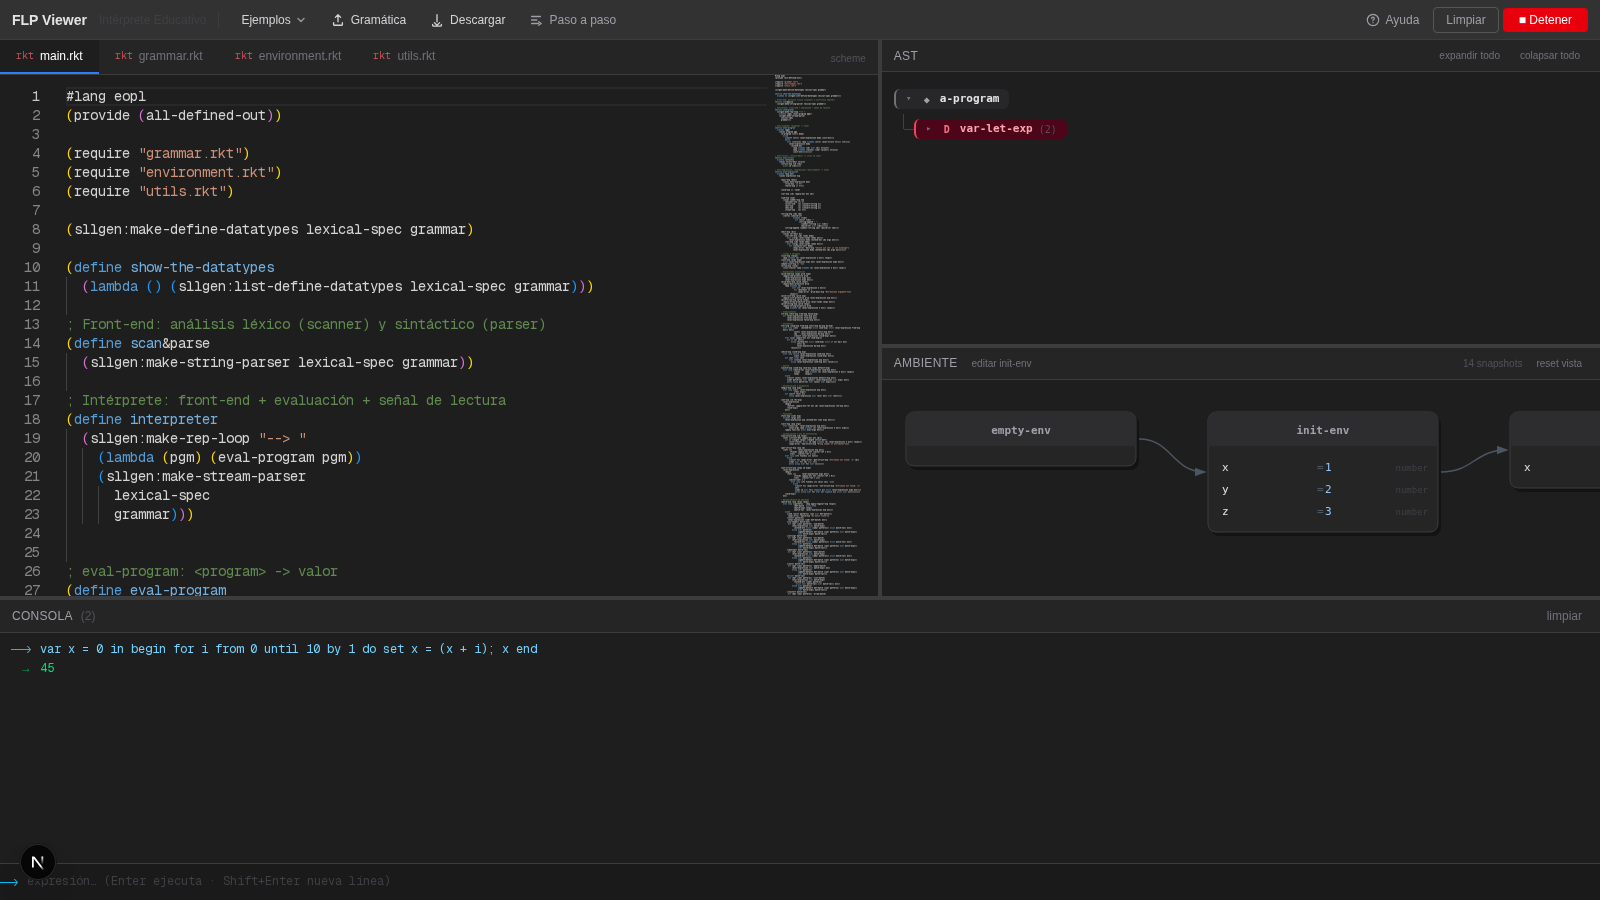
\includegraphics[width=\textwidth]{Capitulo_5/imagenes/cap-06-eval-bucle.png}
    \caption{Evaluación de una expresión con iteración y estado mutable: suma acumulada mediante bucle \texttt{for}}
    \scriptsize \textbf{Fuente:} Elaboración propia
    \label{fig:interfaz-principal}
\end{figure}

\FloatBarrier

La Figura \ref{fig:eval-cierres} evalúa la expresión \texttt{var f = func(x) if (x == 0) \{ 0 else (x + call f((x - 1))) \} in call f(10)}, que define una función recursiva \texttt{f} y la aplica sobre 10, obteniendo la suma triangular 55. A diferencia del caso anterior, el marco final del ambiente contiene la ligadura \texttt{f} cuyo valor es una clausura, lo que permite al estudiante observar que en el modelo de EOPL las funciones son valores de primera clase almacenados en el ambiente como cualquier otra ligadura \cite{Friedman2008EPL}. La presencia de la clausura en el panel de ambiente distingue esta visualización de la anterior y justifica su inclusión como caso complementario.

\begin{figure}[H]
    \centering
    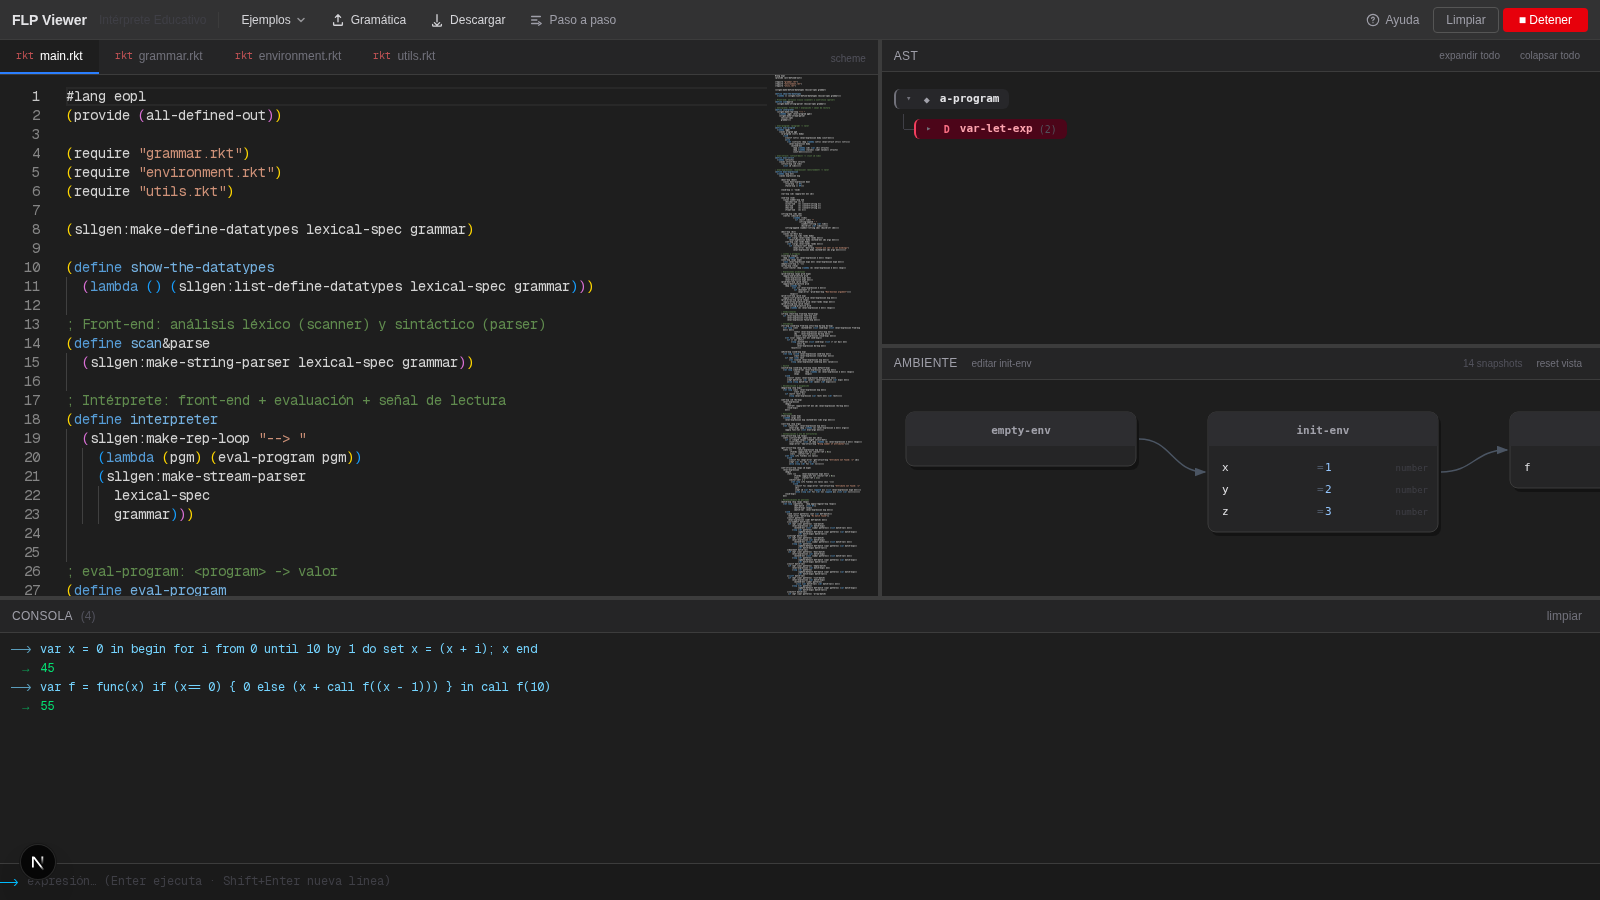
\includegraphics[width=\textwidth]{Capitulo_5/imagenes/cap-07-eval-cierres.png}
    \caption{Evaluación de una función recursiva con clausura: la ligadura \texttt{f} en el panel de ambiente refleja una función como valor de primera clase}
    \scriptsize \textbf{Fuente:} Elaboración propia
    \label{fig:eval-cierres}
\end{figure}

\FloatBarrier

\subsection{Biblioteca de ejemplos predefinidos}

La biblioteca de ejemplos predefinidos (RF-05) comprende seis programas cargados durante el renderizado inicial del servidor mediante \texttt{load-examples.ts} y presentados al estudiante desde el modal de bienvenida. Cada entrada está compuesta por el conjunto completo de archivos del intérprete (\texttt{grammar.rkt}, \texttt{environment.rkt}, \texttt{main.rkt} y \texttt{utils.rkt}), de modo que cualquier ejemplo puede ejecutarse y explorarse de forma inmediata sin modificaciones previas. La Tabla~\ref{tab:biblioteca_ejemplos} presenta la correspondencia entre los ejemplos implementados y los indicadores de logro identificados en el Capítulo~\ref{cap3}.

\begin{table}[H]
\centering
\caption{Biblioteca de ejemplos predefinidos y correspondencia con indicadores de logro}
\label{tab:biblioteca_ejemplos}
\footnotesize
\setlength{\tabcolsep}{4pt}
\begin{tabular}{
  >{\centering\arraybackslash}p{0.4cm}
  >{\raggedright\arraybackslash}p{5.5cm}
  >{\centering\arraybackslash}p{6.5cm}
}
\hline
\textbf{\#} & \textbf{Ejemplo} & \textbf{IL abordados} \\
\hline
1 & Hola Mundo        & IL~1.3.1 \\
2 & Lenguaje LET      & IL~1.1.6, IL~1.2.3 \\
3 & Ambientes         & IL~1.2.6, IL~1.2.7 \\
4 & Procedimientos y clausuras & IL~1.2.6 \\
5 & Estado y asignación      & IL~1.2.6, IL~1.2.7 \\
6 & Intérprete EOPL (avanzado) & IL~1.1.6, IL~1.2.6, IL~1.2.7 \\
\hline
\end{tabular}
\vskip 4pt
\footnotesize\textit{Fuente: elaboración propia a partir del microcurrículo de la asignatura (código 750017C).}
\end{table}

\FloatBarrier

La secuencia responde a dos ejes de variación simultáneos: la complejidad del lenguaje interpretado y la arquitectura del ambiente de ejecución. Los tres primeros ejemplos comparten un ambiente funcional con valores almacenados en listas inmutables; a partir del cuarto, el ambiente introduce celdas mutables mediante el tipo \texttt{a-ref} sobre vectores, cambio arquitectónico en \texttt{environment.rkt} que hace observable la diferencia entre ligadura y asignación \cite{Friedman2008EPL}.

\textit{Hola Mundo} define dos reglas gramaticales (\texttt{print-exp} y \texttt{string-exp}) y dos casos de evaluación, sin ligaduras activas ni operaciones sobre el ambiente, exponiendo el pipeline completo de interpretación en su forma más reducida \cite{Stamenkovic2024AWE}. \textit{Lenguaje LET} implementa el lenguaje homónimo del Capítulo~3 de EOPL \cite{Friedman2008EPL} con siete reglas de producción y seis casos de evaluación; \texttt{let-exp} introduce la primera llamada a \texttt{extend-env}, apilando cada ligadura en un nuevo marco funcional inmutable. \textit{Ambientes} reutiliza la gramática y el evaluador del ejemplo anterior, modificando únicamente \texttt{init-env} para precargar tres ligaduras (\texttt{x=1}, \texttt{y=2}, \texttt{z=3}), lo que permite observar de inmediato la búsqueda por la cadena de marcos y el \textit{shadowing} entre ligaduras homónimas \cite{Sorva2013}.

\textit{Procedimientos y clausuras} extiende el Lenguaje LET con \texttt{proc} y \texttt{call} (lenguaje PROC, Capítulo~3 de EOPL \cite{Friedman2008EPL}); la clausura se implementa como una función Racket que captura el ambiente léxico vigente al evaluar \texttt{proc-exp}, de modo que la invocación posterior extiende ese ambiente capturado y no el activo en el punto de llamada. \textit{Estado y asignación} introduce el lenguaje IMPLICIT-REFS (Capítulo~4 de EOPL \cite{Friedman2008EPL}) mediante un cambio concentrado en \texttt{environment.rkt}: los valores pasan de listas a celdas mutables (\texttt{a-ref} sobre vectores), lo que habilita en \texttt{main.rkt} la operación \texttt{set} vía \texttt{setref!} sin crear un nuevo marco, a diferencia de \texttt{let}. \textit{Intérprete EOPL (avanzado)} combina el modelo de referencias mutables con un lenguaje propio que incorpora estructuras de datos, arreglos, iteradores (\texttt{for}, \texttt{while}), \texttt{switch} y reconocimiento de patrones; la función \texttt{contains-set?} hace cumplir en tiempo de ejecución que las ligaduras \texttt{let} no admitan asignación, y este intérprete sirve como base de las evaluaciones representativas documentadas en las Figuras~\ref{fig:interfaz-principal} y~\ref{fig:eval-cierres}.

\subsection{Punto de acceso de ejecución}

La ruta de API \texttt{/api/run} se implementó como un manejador HTTP POST en \texttt{app/api/run/route.ts}, siguiendo el modelo de rutas de Next.js. Su flujo de operación comprende cuatro fases.

En la primera fase, el servidor crea un directorio temporal exclusivo para la solicitud mediante \texttt{mkdtemp}\footnote{\texttt{mkdtemp} es una llamada del sistema POSIX que crea un directorio temporal con nombre único, garantizando que no colisione con directorios preexistentes aunque varias solicitudes se procesen de forma concurrente.} y escribe en él todos los archivos del editor recibidos en el cuerpo de la petición. Antes de escribir \texttt{environment.rkt} y \texttt{main.rkt}, la función \texttt{injectRuntime} inyecta en su contenido los módulos de instrumentación correspondientes (\texttt{\_tracking.rkt} y \texttt{\_stream-parser.rkt} respectivamente). El archivo \texttt{\_runner.rkt} se copia también al directorio temporal como punto de entrada del proceso Racket.

En la segunda fase, el servidor lanza el proceso Racket sobre \texttt{\_runner.rkt} mediante \texttt{execFile}, pasando la expresión de prueba como argumento y aplicando un tiempo límite de 15 segundos. La señal de cancelación del \texttt{AbortController}\footnote{\texttt{AbortController} es una API web estándar que permite cancelar operaciones asíncronas mediante una señal compartida entre el código que inicia la operación y el que la ejecuta. Cuando el cliente cierra la conexión, la señal se activa y el proceso Racket es terminado antes de consumir el tiempo límite completo.} asociado a la petición permite interrumpir el proceso si el cliente cancela la solicitud antes de que finalice la ejecución.

En la tercera fase, el servidor deserializa la salida estándar del proceso. Si la salida es un arreglo JSON válido, se interpreta como una secuencia de pasos de evaluación. De lo contrario, se trata como texto plano. Los mensajes de error presentes en \texttt{stderr} son normalizados por la función \texttt{cleanStderr}, que elimina las secciones de contexto interno del intérprete Racket que resultan irrelevantes para el estudiante.

En la cuarta fase, el servidor elimina el directorio temporal y retorna la respuesta HTTP con los campos \texttt{steps}, \texttt{stderr} y \texttt{error}. La eliminación del directorio se realiza en el bloque \texttt{finally} del manejador para garantizar la limpieza del sistema de archivos independientemente del resultado de la ejecución.

\subsection{Instrumentación en tiempo de ejecución}

La instrumentación en tiempo de ejecución se implementó mediante tres archivos Racket que se inyectan en el entorno de ejecución de forma transparente para el estudiante.

El archivo \texttt{\_tracking.rkt} redefine la función \texttt{extend-env} al momento de cargar el módulo \texttt{environment.rkt}. Cada llamada a la función redefinida registra un \textit{snapshot} del estado del ambiente en el log interno \texttt{\_env-log}. Al finalizar cada evaluación, el ejecutor principal lee este log e incluye la secuencia de marcos en la respuesta serializada.

El archivo \texttt{\_stream-parser.rkt} se inyecta al final de \texttt{main.rkt} e instrumenta la función de evaluación del programa para capturar, por cada expresión de nivel superior evaluada, el árbol de sintaxis abstracta resultante, el estado del ambiente y el valor producido. La salida se serializa como un arreglo JSON de objetos de paso, donde cada objeto incluye los campos \texttt{ast}, \texttt{environments} y \texttt{output}.

El archivo \texttt{\_runner.rkt} actúa como punto de entrada del proceso Racket. Carga los módulos del proyecto en el orden correcto, recibe la expresión de prueba como argumento de línea de comandos y coordina la evaluación dentro de un manejador de excepciones que captura errores del intérprete y los incluye en la respuesta.

En el flujo de descarga del proyecto, la función \texttt{downloadZip} de \texttt{playground-utils.ts} genera un archivo ZIP con los archivos del editor, eliminando previamente los bloques de instrumentación marcados con las directivas \texttt{FLP-VIEWER-TRACKING-START/END}. Esto garantiza que el código exportado sea directamente compatible con el entorno DrRacket \cite{felleisen2018racket} sin modificaciones adicionales.


\section{Flujo de ejecución principal}

La Figura \ref{fig:secuencia-ejecucion} ilustra el flujo de ejecución que se produce cuando el estudiante envía una expresión desde la consola del prototipo, desde la interacción inicial hasta la obtención del resultado en el servidor. El flujo inicia en el componente \texttt{ConsoleOutput}, que delega la acción al orquestador \texttt{PlaygroundLayout}. Este registra la expresión en el historial, inicializa el mecanismo de cancelación y deshabilita nuevas ejecuciones concurrentes. A continuación, invoca el servicio \texttt{racket.ts}, que empaqueta los archivos del editor y la expresión en una petición HTTP POST hacia \texttt{/api/run}. El servidor de aplicación recibe la solicitud, prepara el entorno de ejecución aislado, lanza el proceso Racket, deserializa su salida y devuelve la secuencia de pasos al cliente.

\begin{figure}[H]
    \centering
    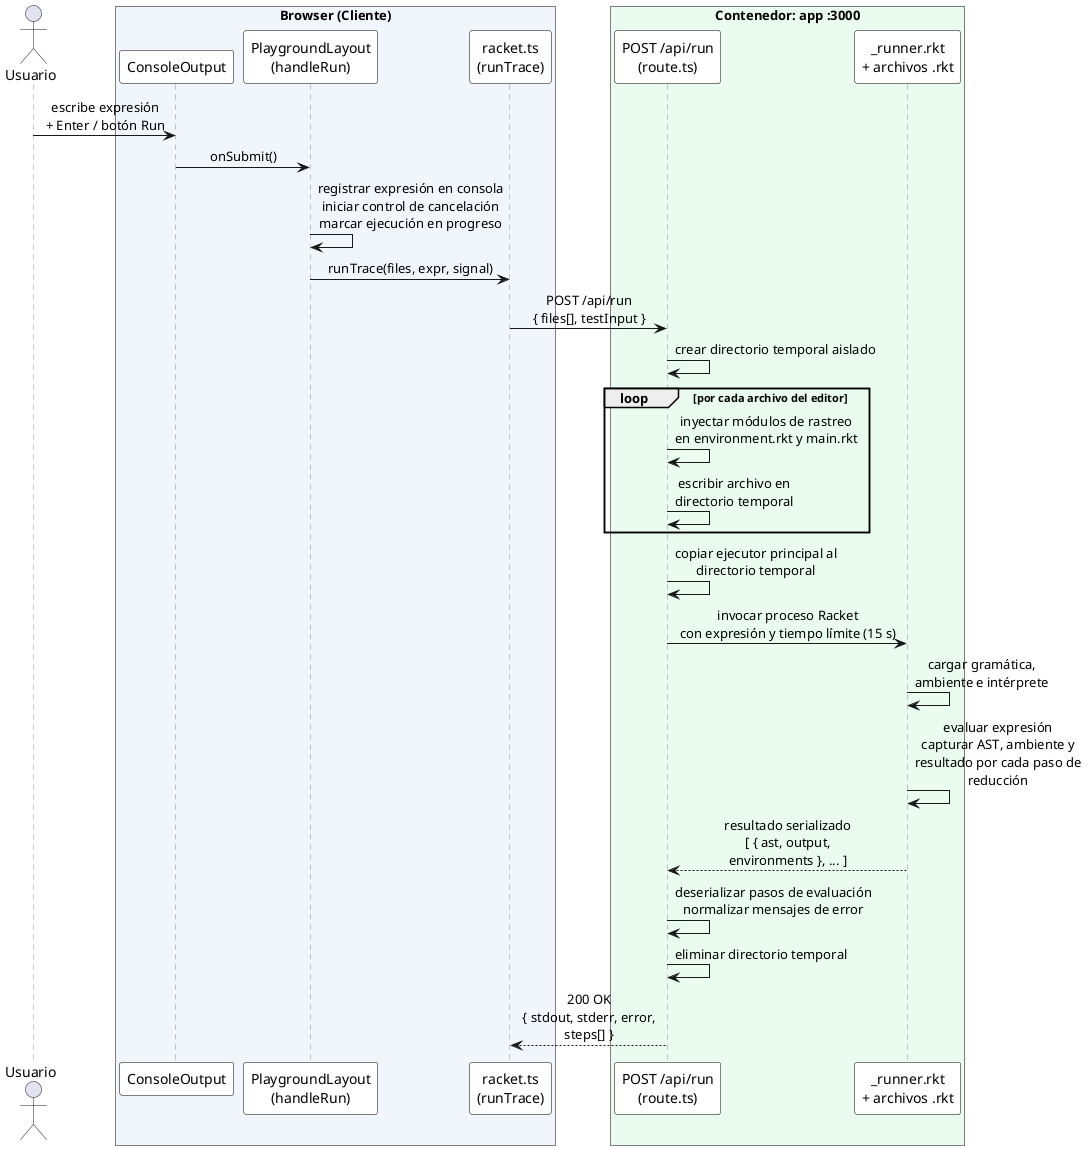
\includegraphics[width=\textwidth,height=0.82\textheight,keepaspectratio]{Capitulo_5/imagenes/secuencia-ejecucion.png}
    \caption{Diagrama de secuencia de la solicitud y evaluación en el servidor del prototipo FLP Viewer}
    \scriptsize \textbf{Fuente:} Elaboración propia
    \label{fig:secuencia-ejecucion}
\end{figure}

\FloatBarrier

Una vez que el cliente recibe la respuesta, \texttt{PlaygroundLayout} distribuye los resultados entre los paneles de visualización según el modo activo, tal como se muestra en la Figura \ref{fig:secuencia-resultado}: en modo normal actualiza el AST, el ambiente y la consola con el estado final, y en modo paso a paso encola los pasos y presenta el primero de forma inmediata, habilitando la navegación manual.

\begin{figure}[H]
    \centering
    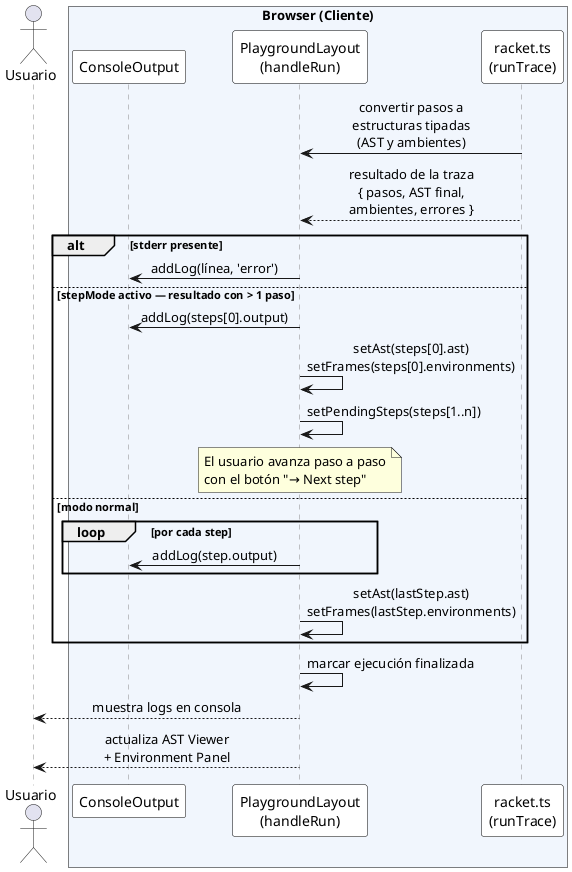
\includegraphics[width=\textwidth,height=0.82\textheight,keepaspectratio]{Capitulo_5/imagenes/secuencia-resultado.png}
    \caption{Diagrama de secuencia de la distribución de resultados en la interfaz del prototipo FLP Viewer}
    \scriptsize \textbf{Fuente:} Elaboración propia
    \label{fig:secuencia-resultado}
\end{figure}

\FloatBarrier


\section{Despliegue en entorno de pruebas}

El prototipo se despliega mediante Coolify \cite{coolify}, una plataforma de despliegue autoalojada que permite gestionar aplicaciones contenerizadas sobre infraestructura propia y construir la imagen de la aplicación directamente a partir del \textit{Dockerfile} del proyecto. Su elección responde a la necesidad de disponer de un mecanismo de despliegue reproducible y centralizado sobre el servidor utilizado para el entorno de pruebas, delegando en la plataforma tareas de infraestructura como el enrutamiento de solicitudes y la gestión de certificados TLS. La Figura \ref{fig:despliegue} presenta el diagrama de la infraestructura de despliegue.

La imagen del contenedor de aplicación se construye mediante un \textit{Dockerfile} multi-etapa con tres etapas diferenciadas. La primera etapa (\texttt{deps}) instala las dependencias del proyecto utilizando \texttt{pnpm} sobre una imagen base de Node.js 25 Alpine. La segunda etapa (\texttt{builder}) ejecuta la construcción de Next.js en modo \textit{standalone}\footnote{El modo \textit{standalone} de Next.js genera un servidor Node.js autocontenido que incluye únicamente las dependencias estrictamente necesarias para producción, sin requerir la carpeta \texttt{node\_modules} completa en el entorno de despliegue. Esto reduce significativamente el tamaño de la imagen Docker resultante.}, que produce un artefacto autocontenido con todas las dependencias necesarias para ejecutar el servidor en producción. La tercera etapa (\texttt{runner}) utiliza la imagen \texttt{node:25-bookworm-slim} e instala el intérprete de Racket como dependencia del sistema operativo mediante \texttt{apt-get}. Esta etapa copia únicamente el artefacto \textit{standalone}, el directorio de archivos estáticos y los tres archivos de instrumentación Racket, minimizando el tamaño de la imagen final. La variable de entorno \texttt{RACKET\_BIN} se configura en \texttt{/usr/bin/racket} para que la ruta de API localice el ejecutable sin depender de la configuración del sistema anfitrión.

El contenedor de la aplicación expone el puerto interno 3000, el cual no se publica directamente hacia el host. Coolify enruta las solicitudes externas hacia este puerto mediante un \textit{reverse proxy}\footnote{Coolify utiliza Traefik como \textit{reverse proxy} por defecto, encargado de dirigir las solicitudes entrantes hacia el contenedor correspondiente según el dominio configurado y de gestionar de forma automática los certificados TLS mediante Let's Encrypt \cite{coolify_traefik}.} que gestiona de forma automática, sin requerir la definición manual de reglas de enrutamiento en el proyecto. Esta arquitectura garantiza que el acceso externo al prototipo se realice exclusivamente a través del proxy, centralizando el control de las solicitudes entrantes.

\begin{figure}[H]
    \centering
    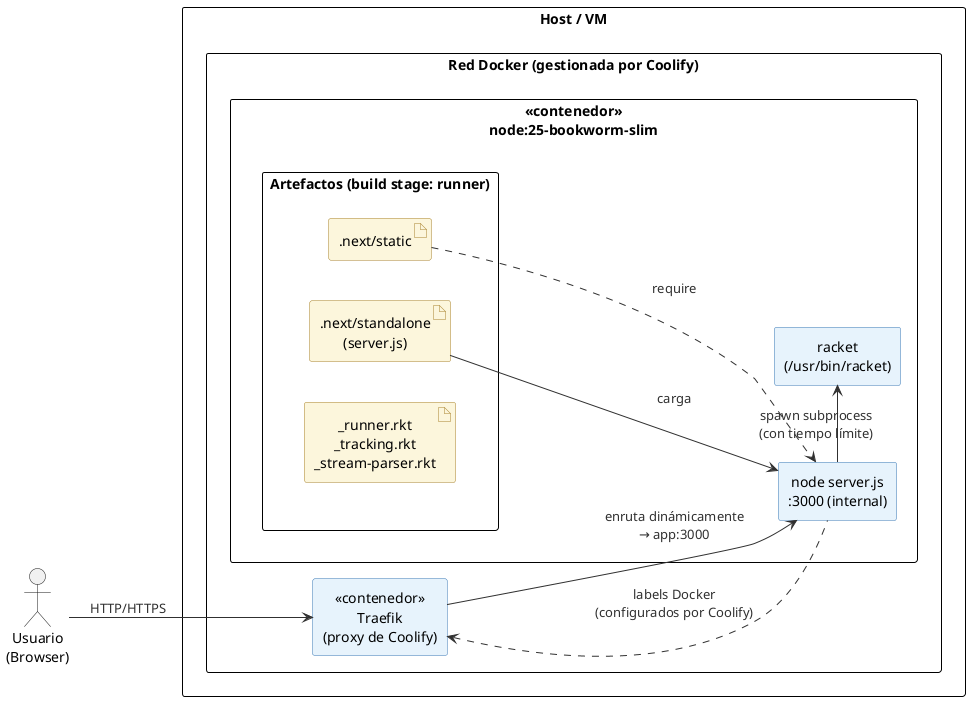
\includegraphics[width=0.85\textwidth]{Capitulo_5/imagenes/despliegue.png}
    \caption{Diagrama de despliegue del prototipo FLP Viewer en el entorno de pruebas}
    \scriptsize \textbf{Fuente:} Elaboración propia
    \label{fig:despliegue}
\end{figure}

\FloatBarrier


\section{Verificación de requisitos funcionales}

La Tabla \ref{tab:verificacion_rf} presenta la correspondencia entre los requisitos funcionales definidos en el diseño y los módulos que materializan cada uno en la implementación. Todos los requisitos de prioridad alta y media definidos en la especificación fueron implementados en el prototipo entregado.

\begin{table}[H]
\centering
\caption{Verificación del cumplimiento de los requisitos funcionales}
\label{tab:verificacion_rf}
\footnotesize
\setlength{\tabcolsep}{4pt}
\begin{tabular}{
  >{\centering\arraybackslash}p{1.2cm}
  >{\raggedright\arraybackslash}p{3.8cm}
  >{\raggedright\arraybackslash}p{6.8cm}
  >{\centering\arraybackslash}p{2.1cm}
}
\hline
\textbf{ID} & \textbf{Nombre} & \textbf{Módulos de implementación} & \textbf{Estado} \\
\hline
RF-01 & Generación del AST &
  \texttt{\_runner.rkt}, \texttt{\_stream-parser.rkt}, \texttt{racket.ts} &
  Implementado \\
RF-02 & Visualización del AST &
  \texttt{ASTViewer.tsx}, \texttt{PlaygroundLayout.tsx} &
  Implementado \\
RF-03 & Ejecución y evaluación &
  \texttt{app/api/run/route.ts} (\textit{endpoint} \texttt{/api/run}) &
  Implementado \\
RF-04 & Representación del ambiente &
  \texttt{\_tracking.rkt}, \texttt{EnvironmentPanel.tsx} &
  Implementado \\
RF-05 & Biblioteca de ejemplos &
  \texttt{examples/}, \texttt{load-examples.ts}, \texttt{WelcomeModal.tsx} &
  Implementado \\
RF-06 & Validación de sintaxis Racket &
  \texttt{bnf-lexer.ts}, \texttt{bnf-parser.ts}, \texttt{cleanStderr()} en \texttt{route.ts} &
  Implementado \\
RF-07 & Visualización del intérprete &
  \texttt{EditorPanel.tsx}, \texttt{CodeEditor.tsx} (líneas bloqueadas con Monaco Editor) &
  Implementado \\
RF-08 & Plantilla base y exportación &
  \texttt{INITIAL\_FILES} y \texttt{downloadZip()} en \texttt{playground-utils.ts} &
  Implementado \\
\hline
\end{tabular}
\vskip 4pt
\footnotesize\textit{Fuente: elaboración propia.}
\end{table}

\FloatBarrier


\section{Evaluación de la calidad del software}

Con el propósito de complementar la verificación funcional presentada en la sección anterior con una valoración de la calidad técnica del código fuente, se realizó un análisis estático del prototipo FLP Viewer mediante SonarCloud. Esta evaluación permite identificar problemas relacionados con confiabilidad, seguridad, mantenibilidad, duplicación de código y cobertura de las pruebas automatizadas, aspectos que no son observables a través de la verificación de requisitos funcionales descrita previamente.

SonarCloud es una plataforma de análisis continuo de código fuente que examina un proyecto en busca de errores (\textit{bugs}), vulnerabilidades, \textit{code smells}\footnote{Patrones de código que, sin constituir errores funcionales, incrementan la deuda técnica y dificultan el mantenimiento del software.} y fragmentos duplicados, además de integrar los resultados de cobertura generados por las pruebas automatizadas del proyecto. Sobre estas métricas, la plataforma aplica \textit{Quality Gates}, definidos como un conjunto de condiciones que se evalúan sobre los resultados de cada análisis para determinar si el código cumple un nivel mínimo de calidad. El \textit{Quality Gate} se reporta como aprobado cuando los resultados satisfacen dichas condiciones, y como no aprobado en caso contrario \cite{sonarcloud_quality_gates}.

Para la evaluación del prototipo, el repositorio de FLP Viewer se integró con SonarCloud y se ejecutó el análisis sobre la rama principal (\texttt{main}) una vez finalizado el desarrollo de las funcionalidades contempladas, con el propósito de obtener una medición del estado final del código. La Figura \ref{fig:sonarcloud} presenta el panel de resultados generado por la plataforma, y la Tabla \ref{tab:sonarcloud-resultados} resume los valores obtenidos para cada métrica.

\begin{figure}[H]
    \centering
    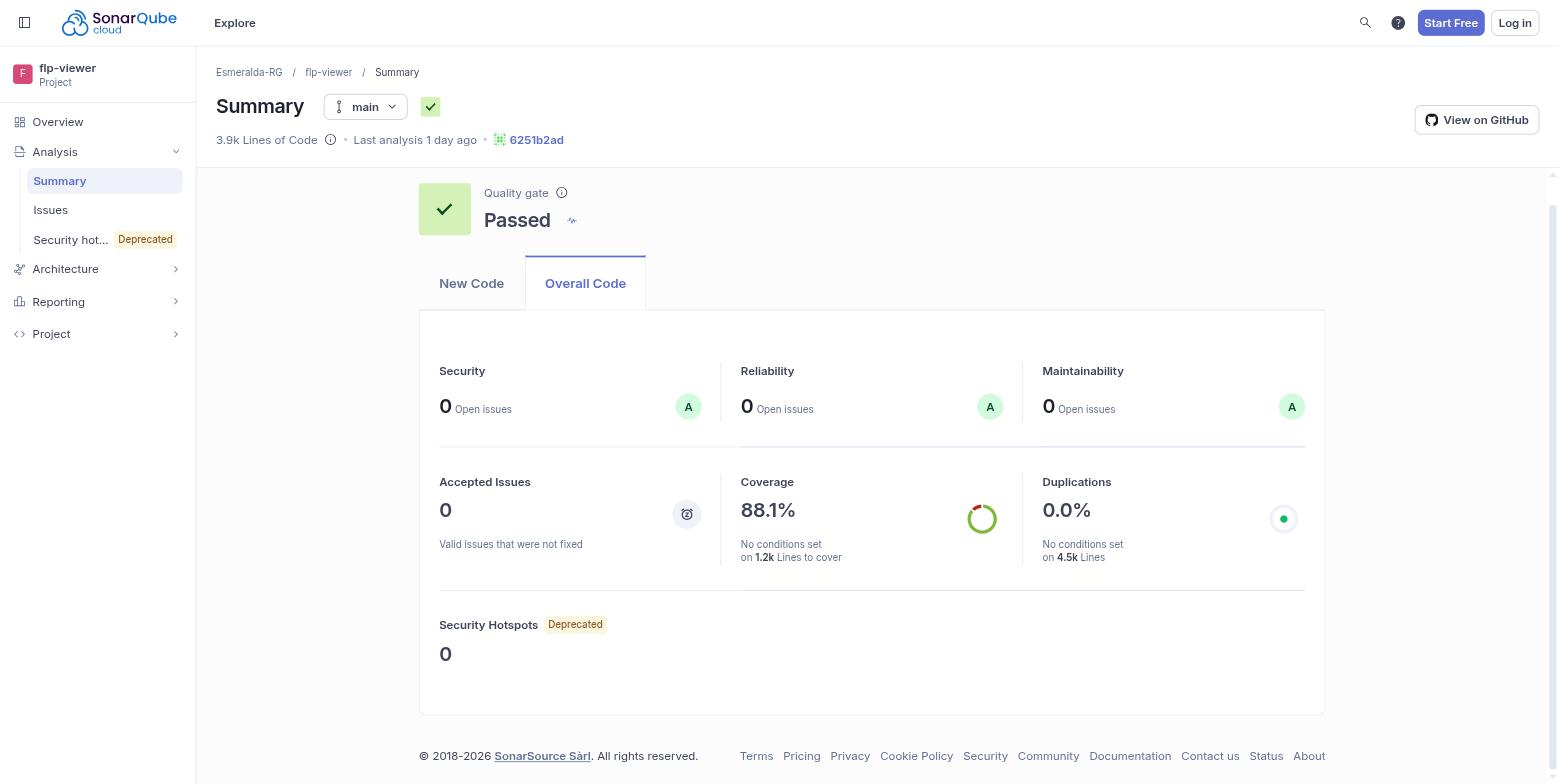
\includegraphics[width=0.85\textwidth]{Capitulo_5/imagenes/sonarcloud-resumen.jpg}
    \caption{Panel de resultados del análisis de calidad del prototipo FLP Viewer en SonarCloud}
    \scriptsize \textbf{Fuente:} SonarCloud, rama \texttt{main} del repositorio del proyecto
    \label{fig:sonarcloud}
\end{figure}

\begin{table}[H]
\centering
\footnotesize
\caption{Resultados del análisis de calidad del prototipo FLP Viewer mediante SonarCloud}
\label{tab:sonarcloud-resultados}
\begin{tabular}{|l|c|}
\hline
\textbf{Métrica} & \textbf{Resultado} \\
\hline
Quality Gate & Aprobado \\
\hline
Bugs & 0 \\
\hline
Vulnerabilidades & 0 \\
\hline
Code Smells & 0 \\
\hline
Security Hotspots & 0 \\
\hline
Duplicación de código & 0.0\,\% \\
\hline
Cobertura de código & 88.1\,\% \\
\hline
Reliability Rating & A \\
\hline
Security Rating & A \\
\hline
Maintainability Rating & A \\
\hline
\end{tabular}
\vskip 4pt
\footnotesize\textit{Fuente: elaboración propia, a partir del análisis de SonarCloud sobre la rama \texttt{main} del repositorio\footnote{\url{https://sonarcloud.io/summary/overall?id=Esmeralda-RG_flp-viewer&branch=main}}.}
\end{table}

La cobertura obtenida, del 88.1\,\%, indica la proporción del código ejecutable del prototipo que fue ejercitada mediante las pruebas automatizadas del proyecto. Esta métrica permite identificar qué partes del código fueron efectivamente recorridas durante las pruebas y, en consecuencia, detectar zonas que podrían requerir casos de prueba adicionales \cite{sonarcloud_coverage}. Las calificaciones de confiabilidad, seguridad y mantenibilidad obtenidas corresponden en los tres casos al nivel A, el más favorable de la escala empleada por SonarCloud, en la cual el nivel A de confiabilidad y de seguridad se asigna cuando el análisis no reporta errores ni vulnerabilidades, respectivamente, y el nivel A de mantenibilidad se asigna cuando la deuda técnica estimada no supera el 5\,\% del esfuerzo de desarrollo del código analizado \cite{sonarcloud_metrics}. De manera consistente con estas calificaciones, el análisis no reportó \textit{code smells}, \textit{security hotspots} pendientes de revisión ni fragmentos de código duplicados, y el proyecto satisfizo las condiciones del \textit{Quality Gate} \textit{Sonar way} aplicado, por lo que el resultado global del análisis se reportó como aprobado.

Estos resultados deben interpretarse dentro del alcance del análisis realizado. El hecho de que SonarCloud no reporte errores ni vulnerabilidades en el código analizado no implica que el prototipo esté libre de defectos, sino que el código no presentó, al momento de la evaluación, incidencias frente a las reglas de análisis estático aplicadas por la herramienta. De manera análoga, la cobertura reportada refleja qué proporción del código fue ejercitada por las pruebas existentes, sin constituir por sí sola una medida de la corrección funcional del sistema. En conjunto, los resultados obtenidos constituyen evidencia favorable respecto a la calidad técnica del código del prototipo, particularmente en lo referente a la ausencia de duplicación, la cobertura de pruebas alcanzada y las calificaciones de confiabilidad, seguridad y mantenibilidad, en el contexto de un prototipo de alcance acotado de aproximadamente 3\,900 líneas de código.

\FloatBarrier

